\section{Settings and Feedback}
\label{prototype:SettingsAndFeedback}

To make it easier to alter user settings and gather feedback from users I have created a settings tab and a feedback tab. The settings tab allows users to change preferences such as whether extensions are enabled, whether personal information is hidden in screenshots, and other user-specific settings. The feedback tab provides a simple way for users to submit their thoughts and suggestions about the app, which is crucial for ongoing development and improvement. Both of these tabs are designed to be easily accessible from the options area of the app, and are fully functional however there are some movile device issues i need to revovle such as long feedback form flowing off the page (producing a scrollbar) and it being possible to get stuck in the setting subpage (specifically the 'extensions' subpage) without being able to return to the main settings page. These issues will be resolved in future iterations of the app.

\begin{figure}[H]
    \centering
    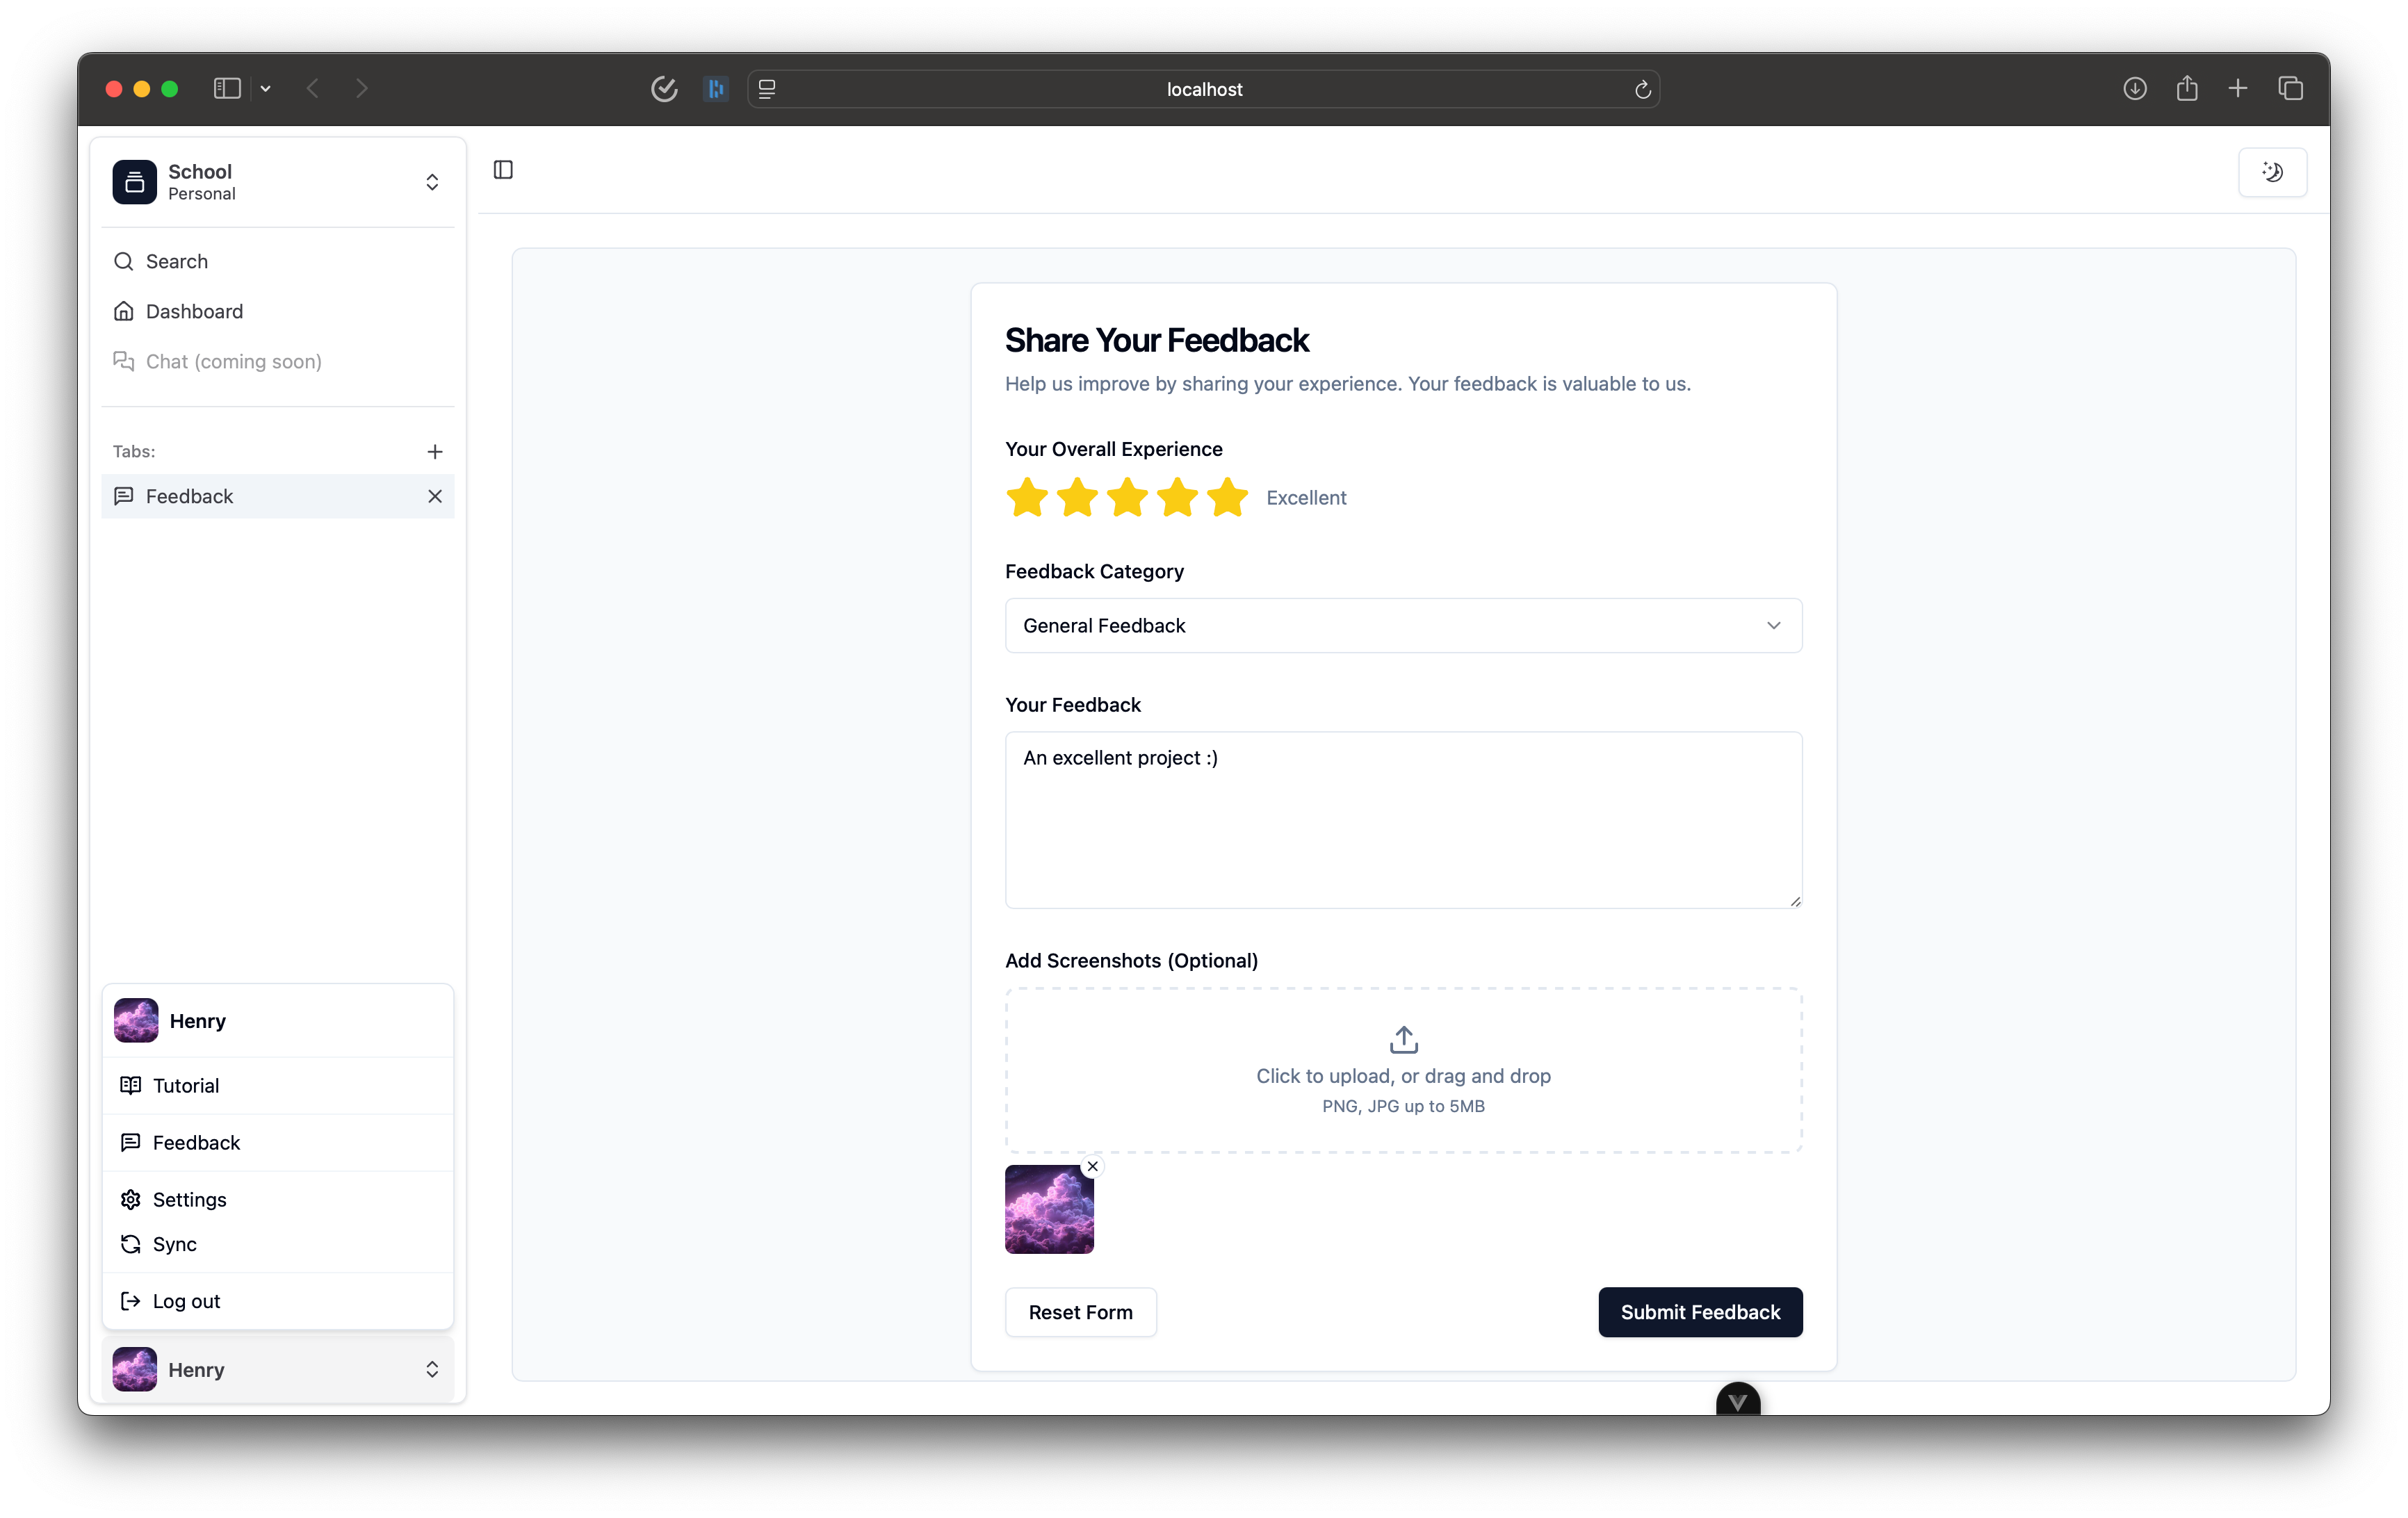
\includegraphics[width=0.8\textwidth]{Prototype/23_SettingsAndFeedback/media/feedback.png}
    \caption{Feedback Form}
    \label{fig:settings_and_feedback}
\end{figure}

\begin{figure}[H]
    \centering
    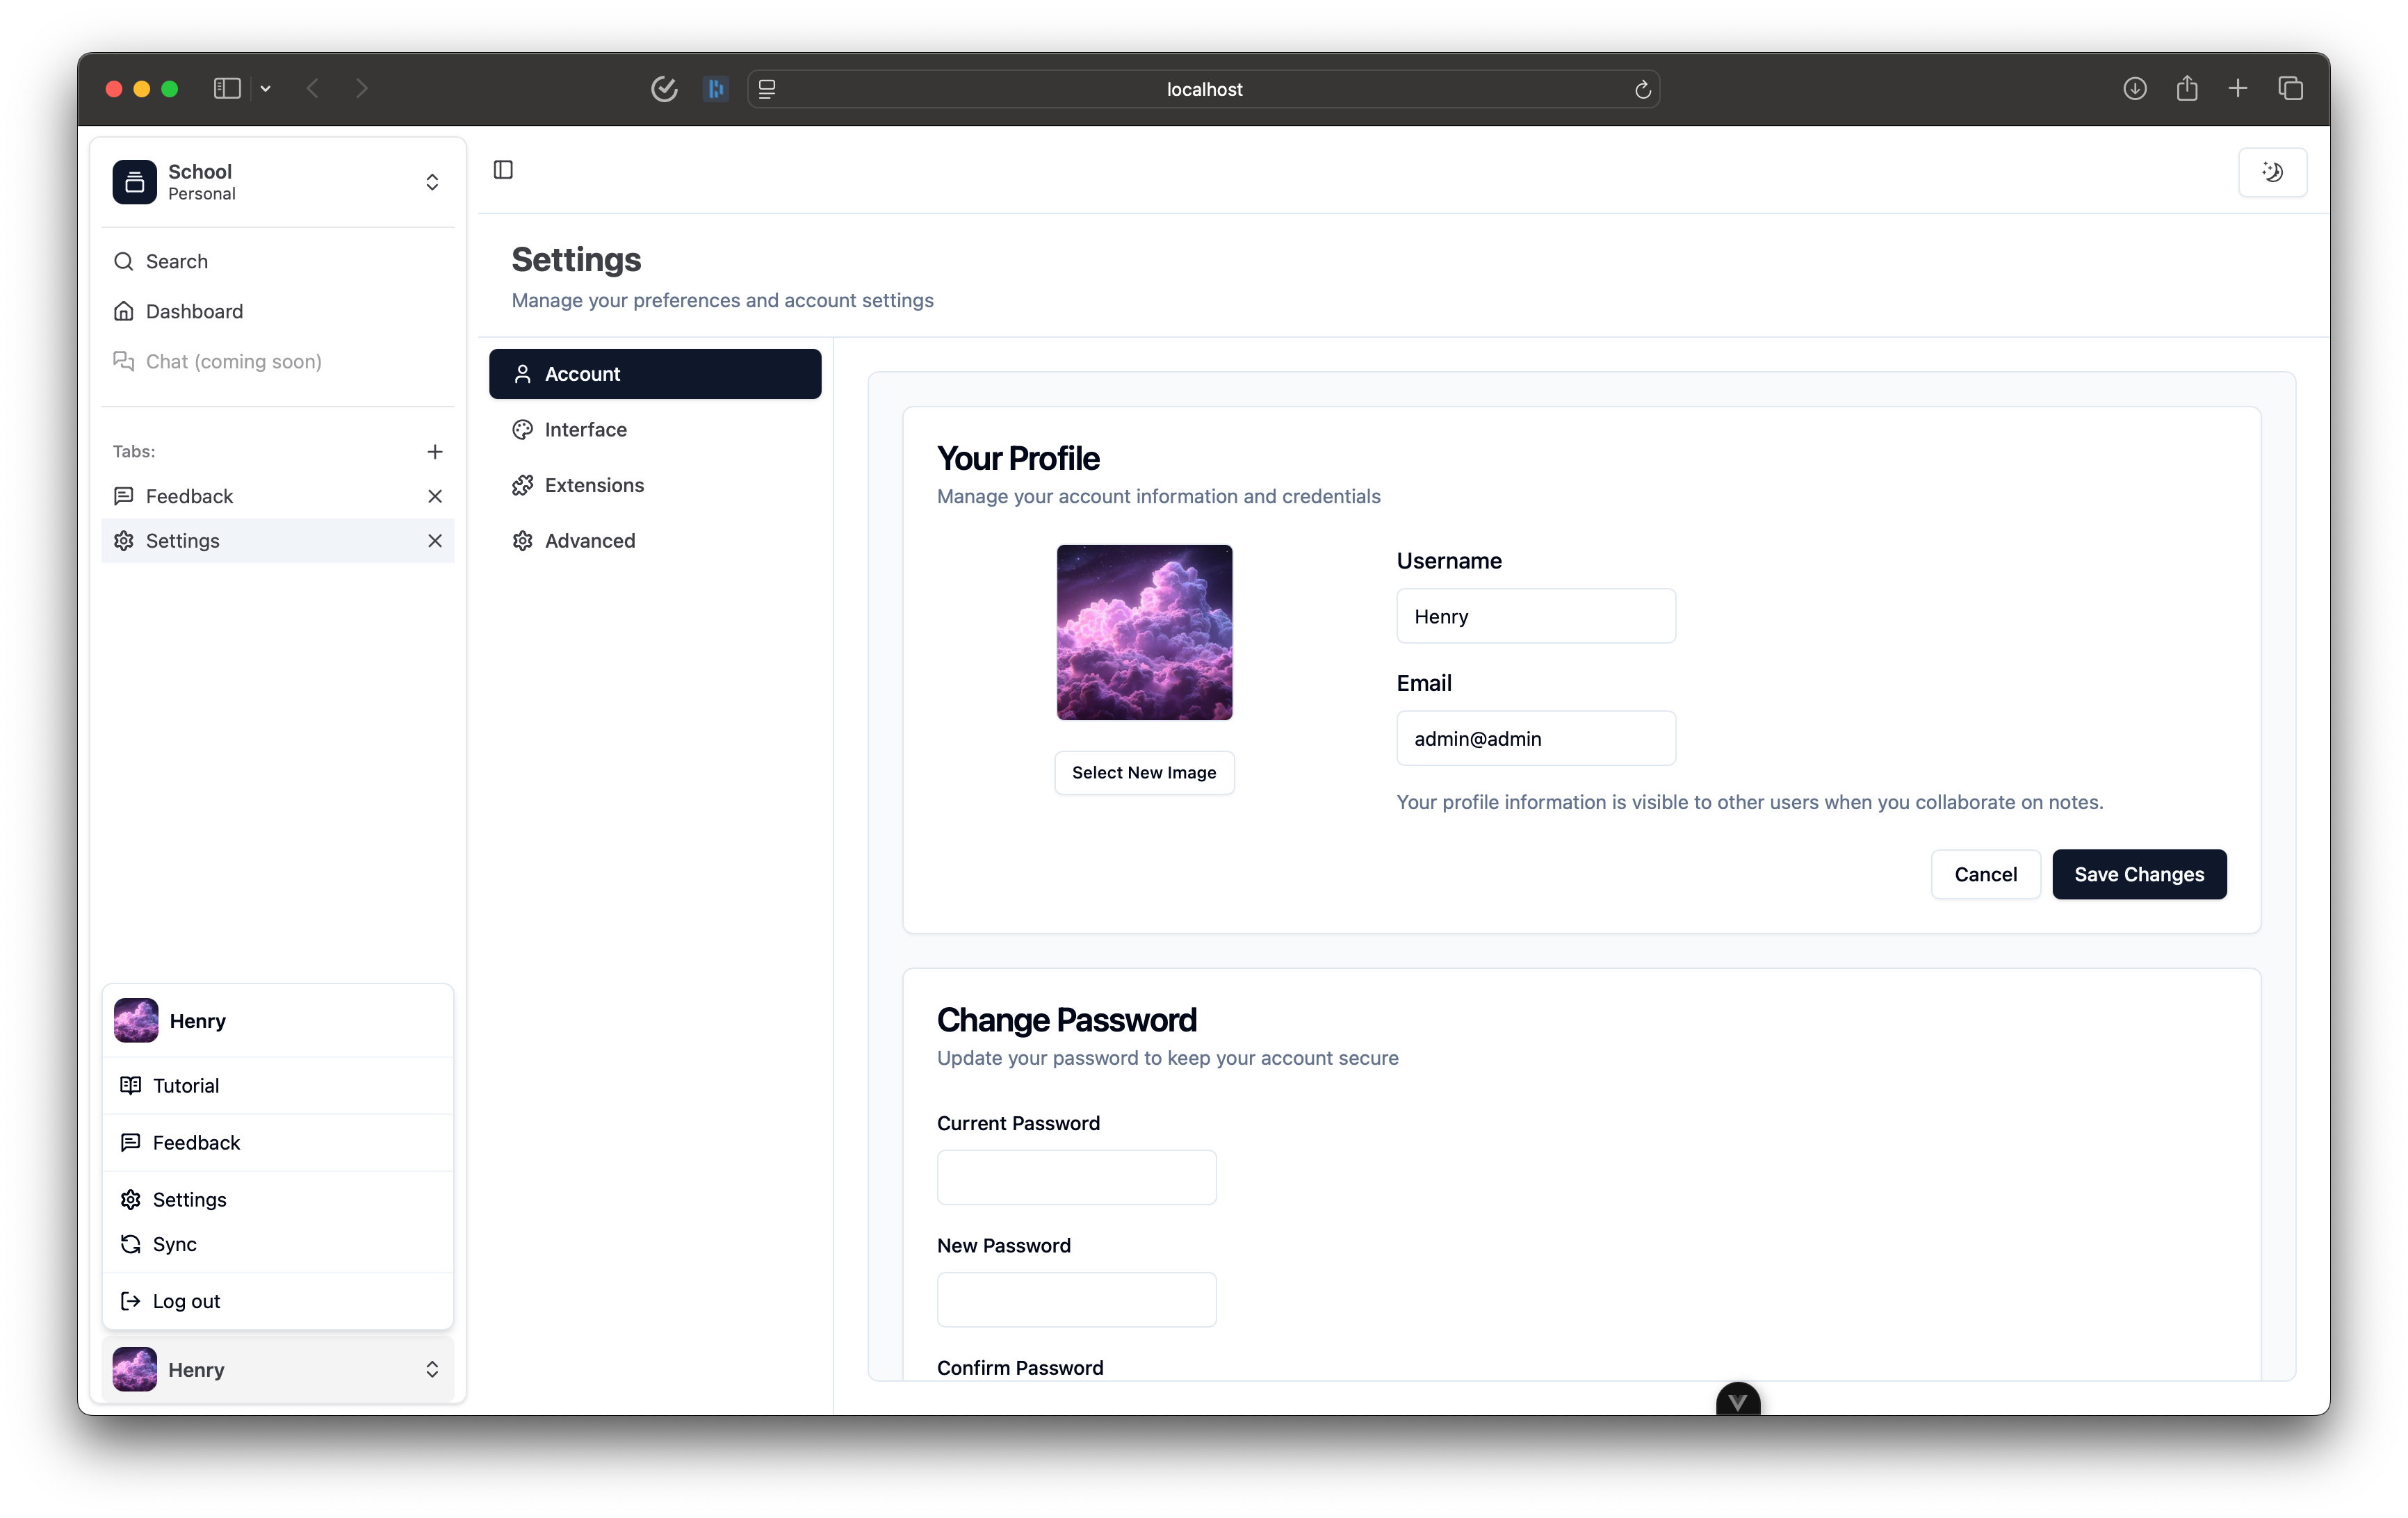
\includegraphics[width=0.8\textwidth]{Prototype/23_SettingsAndFeedback/media/settings.png}
    \caption{Settings Tab}
    \label{fig:settings_and_feedback}
\end{figure}